\documentclass[10pt]{article}
\usepackage[letterpaper,landscape,margin=0.55in]{geometry}
\usepackage{graphicx}
\usepackage{amsmath}
\usepackage[T1]{fontenc}
\usepackage{hyperref}
\hypersetup{pdftitle={Order-five trace kernel: Lean proof boundary for FROB C5}}
\setlength{\parindent}{0pt}
\setlength{\parskip}{0.5em}
\begin{document}
\begin{center}
{\Large Order-five trace kernel: Lean proof boundary for FROB C5}\\
22 October 2026 \quad EXP-FROB-91ee9c \quad TASK-20261022-adb94b
\end{center}

\textbf{Proved proposition.} Over any field $R$ and $R$-vector space $V$,
let $F$ be a linear endomorphism with $F^5=1$ and $5\ne0$ in $R$.
For $T(F)=1+F+F^2+F^3+F^4$, Lean proves
$\ker T(F)=\operatorname{range}(F-1)$ and
$\operatorname{Fix}(F)\cap\ker T(F)=\{0\}$.
The proof source is \texttt{formal/CryptoResearch/FrobTrace/OrderFive.lean};
the frozen target is \texttt{formal/targets/frob-c5-order-five-trace-kernel.yaml}.

\begin{center}
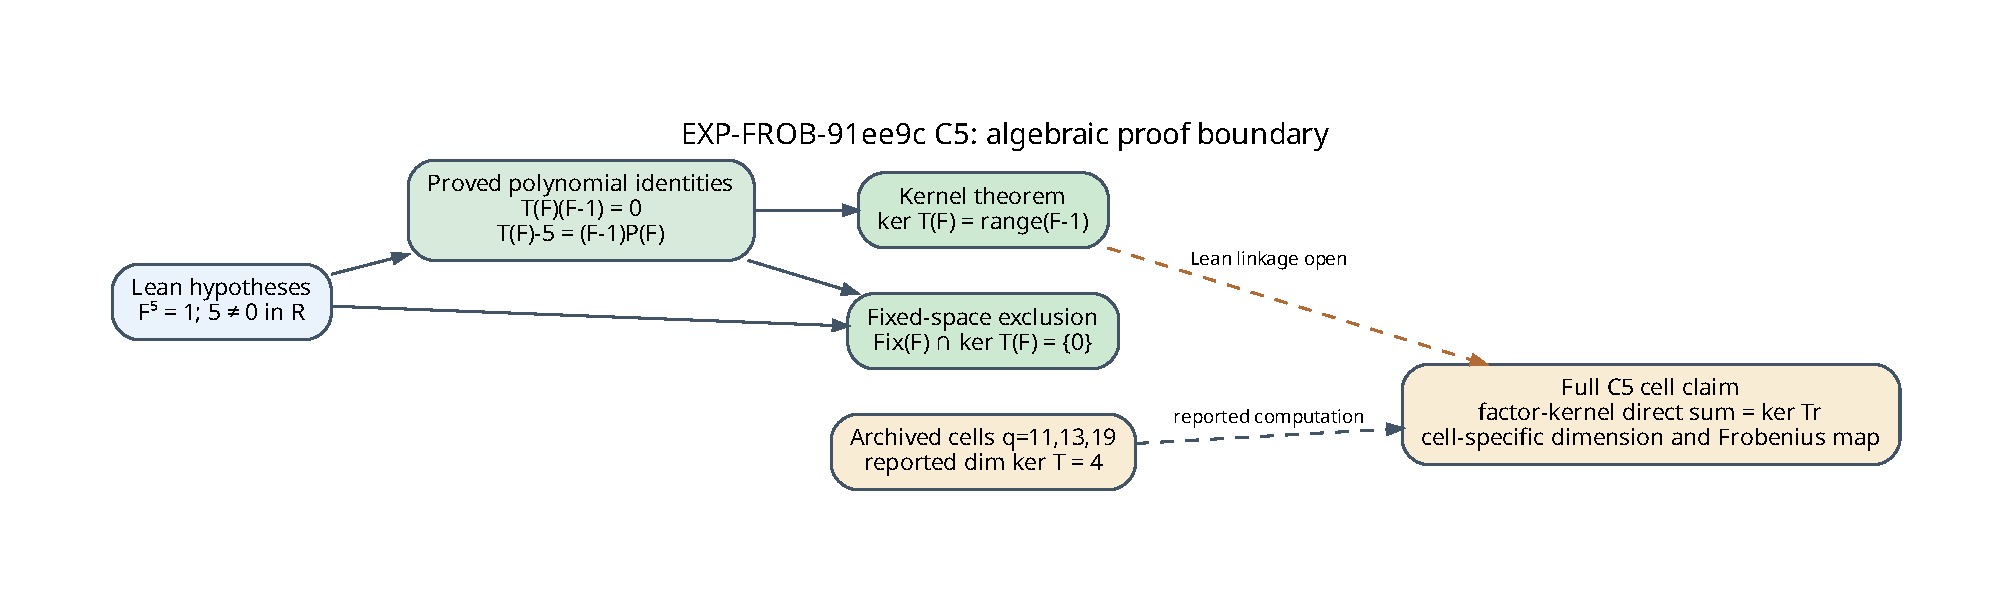
\includegraphics[width=0.97\textwidth,height=0.55\textheight,keepaspectratio]{trace-figure.pdf}
\end{center}

\textbf{Boundary.} The theorem does not construct the archived $q=11,13,19$
finite fields, identify $F$ with their Frobenius maps, prove the reported
dimension four, or prove the nontrivial factor-kernel direct sum. Those are
separate C5 obligations. C8's independent control-arm recheck also remains
open. No performance or attack-cost claim follows from this lemma.

\textbf{Sources.} EXP-FROB-91ee9c \texttt{specification.yaml} control C5;
\texttt{analysis.md} Section 0; frozen
\texttt{TASK-20260914-7119f2/report.md}; 2026-10-22 provenance audit.
\end{document}
